\documentclass[journal=esthag,manuscript=article]{achemso}
%%%%%%%%%%%%%%%%%%%%%%%%%%%%%%%%%%%%%%%%%%%%%%%%%%%%%%%%%%%%%%%%%%%%%
%% Place any additional packages needed here.  Only include packages
%% which are essential, to avoid problems later. Do NOT use any
%% packages which require e-TeX (for example etoolbox): the e-TeX
%% extensions are not currently available on the ACS conversion
%% servers.
%%%%%%%%%%%%%%%%%%%%%%%%%%%%%%%%%%%%%%%%%%%%%%%%%%%%%%%%%%%%%%%%%%%%%
\usepackage[T1]{fontenc}       % Use modern font encodings
\usepackage[utf8]{inputenc}
\usepackage{amsmath}
\usepackage{enumerate}
\pdfminorversion=4
\usepackage{lineno}
% \usepackage{todonotes}

%%%%%%%%%%%%%%%%%%%%%%%%%%%%%%%%%%%%%%%%%%%%%%%%%%%%%%%%%%%%%%%%%%%%%
%% If issues arise when submitting your manuscript, you may want to
%% un-comment the next line.  This provides information on the
%% version of every file you have used.
%%%%%%%%%%%%%%%%%%%%%%%%%%%%%%%%%%%%%%%%%%%%%%%%%%%%%%%%%%%%%%%%%%%%%
\listfiles

%%%%%%%%%%%%%%%%%%%%%%%%%%%%%%%%%%%%%%%%%%%%%%%%%%%%%%%%%%%%%%%%%%%%%
%% Place any additional macros here.  Please use \newcommand* where
%% possible, and avoid layout-changing macros (which are not used
%% when typesetting).
%%%%%%%%%%%%%%%%%%%%%%%%%%%%%%%%%%%%%%%%%%%%%%%%%%%%%%%%%%%%%%%%%%%%%
%% \newcommand*\mycommand[1]{\texttt{\emph{#1}}}


%%%%%%%%%%%%%%%%%%%%%%%%%%%%%%%%%%%%%%%%%%%%%%%%%%%%%%%%%%%%%%%%%%%%%
\author{Eduard Szöcs}
\affiliation[Institute for Environmental Sciences]{Institute for Environmental Sciences, University of Koblenz-Landau, Germany}
\email{szoecs@uni-landau.de}
\phone{+49 (0)6341 280 31552}

\author{Marvin Brinke}
\affiliation[German Federal Institute of Hydrology]{German Federal Institute of Hydrology (BfG), Koblenz, Germany}

\author{Bilgin Karaoglan}
\affiliation[German Environment Agency]{German Environment Agency (UBA), Dessau-Roßlau, Germany}

\author{Ralf B. Schäfer}
\affiliation[University Koblenz-Landau]{Institute for Environmental Sciences, University of Koblenz-Landau, Germany}


%%%%%%%%%%%%%%%%%%%%%%%%%%%%%%%%%%%%%%%%%%%%%%%%%%%%%%%%%%%%%%%%%%%%%
\title[Pesticides small streams]{Large scale risks from agricultural pesticides in small streams}
% \abbreviations{mo, neon, ra, tu, fw}
\keywords{Monitoring, Neonicotinoid, Risk Assessment, Exposure, Freshwater}


%%%%%%%%%%%%%%%%%%%%%%%%%%%%%%%%%%%%%%%%%%%%%%%%%%%%%%%%%%%%%%%%%%%%%
\begin{document}
%%%%%%%%%%%%%%%%%%%%%%%%%%%%%%%%%%%%%%%%%%%%%%%%%%%%%%%%%%%%%%%%%%%%%
%% The "tocentry" environment can be used to create an entry for the
%% graphical table of contents. It is given here as some journals
%% require that it is printed as part of the abstract page. It will
%% be automatically moved as appropriate.
%%%%%%%%%%%%%%%%%%%%%%%%%%%%%%%%%%%%%%%%%%%%%%%%%%%%%%%%%%%%%%%%%%%%%


%%%%%%%%%%%%%%%%%%%%%%%%%%%%%%%%%%%%%%%%%%%%%%%%%%%%%%%%%%%%%%%%%%%%%

\linenumbers

\begin{abstract}
% 150-200 words
Small streams are important refugia for biodiversity.
In agricultural areas they may be at risk from pesticide pollution. 
However, most related studies have been limited to a few streams on the regional level, hampering extrapolation to larger scales. 
We quantified risks as exceedances of regulatory acceptable concentrations (RACs) and used German monitoring data to quantify the drivers thereof and to assess current risks in small streams on a large scale. 
The data set comprised of 1,766,104 measurements of 478 pesticides (including metabolites) related to 24,743 samples from 2,301 sampling sites. 
We investigated the influence of agricultural land use, catchment size, as well as precipitation and seasonal dynamics on pesticide risk taking also concentrations below the limit of quantification into account. 
The exceedances of risk thresholds dropped 3.7-fold at sites with no agriculture, indicating that agricultural land use is a major contributor of pesticides in streams.
Precipitation increased detection probability by 43\% and concentrations were the highest from April to June. 
RACs were exceeded in 26\% of streams.
We found the highest exceedances for neonicotinoid insecticides. 
We conclude that pesticides from agricultural land use are a major threat to small streams and their biodiversity. 
To reflect peak concentrations, current pesticide monitoring needs refinement.

\end{abstract}


% \begin{tocentry}

\section{TOC Art}

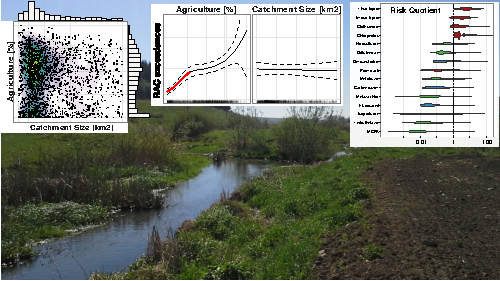
\includegraphics[width=3.33in, height=1.875in]{abstract.pdf}


% \end{tocentry}

%%%! Check all numbers
%%%! Check all references to supplement


%% -------------------------------------------------------------------------
\section{Introduction}
More than 50\% of the total land area in Germany is used by agriculture \citep{statistisches_bundesamt_bodenflache_2014}.
In the year 2014 more than 45,000 tonnes of 776 authorised plant protection products were sold for application on this area \citep{bundesamt_fur_verbraucherschutz_und_lebensmittelsicherheit_absatz_2015}.
The applied pesticides may enter surface waters via spray-drift, edge-of-field run-off or drainage \citep{stehle_probabilistic_2013,schulz_comparison_2001,liess_determination_1999}.
Once entered the surface waters they may have adverse effects on biota and ecosystem functioning \citep{schafer_thresholds_2012}. 
Although it is known that pesticide pollution and its ecological effects increase with the fraction of agricultural land use in the catchment \citep{schulz_field_2004}, the shape of the relationship is unknown and studies on potential thresholds are lacking.

Two recent studies indicate that pesticide concentrations in streams might threaten freshwater biodiversity in the European union.
\citet{malaj_organic_2014} analysed data supplied to the European Union (EU) in the context of the Water Framework Directive (WFD) and showed that almost half of European water bodies are at risk from pesticides.
\citet{stehle_pesticide_2015} compiled 1,566 measured concentrations of 23 insecticides in the EU from scientific publications and found considerable exceedances of regulatory acceptable concentrations (RAC).
However, these studies reflect only a small amount of potentially available data (173 sites in predominantly mid-sized and large rivers in \citet{malaj_organic_2014} and 138 measurements in \citet{stehle_pesticide_2015}), and it is unclear how representative they are for Germany. % 173 estimated from digitized figure C.3 in Malaj 2014; Stehle: Table 2.
Much more comprehensive data on thousands of sites are available from national monitoring programs that are setup for the surveillance of water quality,
which is done independently by the federal states in Germany in compliance with the WFD \citep{quevauviller_water_2008}. 
Despite that these data are providing the opportunity to study pesticide risks and other research questions on a large scale with high spatial density, to date these data have not been compiled.

Small streams comprise a major fraction of streams \citep{nadeau_hydrological_2007}, accommodate a higher proportion of biodiversity compared to larger streams \citep{davies_comparison_2008, biggs_report_2014} and play an important role in the recolonization of disturbed downstream reaches \citep{liess_analyzing_2005, orlinskiy_forested_2015}.
Nevertheless, a clear definition of small streams in terms of catchment or stream size is currently lacking \citep{lorenz_specifics_2016}. 
For example, the WFD defines small streams with a catchment size between 10 and 100 km\textsuperscript{2}, without further categorisation of streams \textless 10km\textsuperscript{2} and \citet{lorenz_specifics_2016} defines small streams with catchment size \textless 10km\textsuperscript{2}. 
Moreover, small streams might particularly be at high risk of pesticide contamination in case of adjacent agricultural areas and given their low dilution potential \citep{schulz_field_2004,liess_determination_1999}.
Indeed, meta-analyses using data from studies with a few sites reported higher pesticide pollution in smaller streams compared to bigger streams \citep{stehle_pesticide_2015,schulz_field_2004}. 
Despite their ecological relevance and potentially higher pesticide exposure, a recent review of pesticide studies showed that a disproportionally small fraction of studies was conducted in small water bodies, and these were largely limited to a few sites \citep{lorenz_specifics_2016}. 
Consequently, knowledge on the pesticide pollution of small streams on larger scales is scant. 
In European law, the Directive 2009/128/EC \citep{European_Union_2009} places an obligation on the EU Member States to adopt National Action Plans (NAP) for the Sustainable Use of Plant Protection Products and the German NAP also addresses the knowledge gap concerning pesticide impact on small streams, specifically including those with catchment size \textless 10km\textsuperscript{2}.

The aim of this study is to identify drivers and dynamics of pesticide concentrations in streams on large spatial scales.
To achieve this, we compiled and analysed large-scale pesticide monitoring data from small streams in Germany and examined four hypotheses:
1) A major fraction of pesticides is applied to agricultural fields.
Therefore, we hypothesised that the most frequent exceedances of RACs occur in streams with a high proportion of agricultural land use in the catchment. 
If agricultural land use was indeed the main source for pesticides in streams, the RAC exceedances should drop to negligible levels in the absence of agricultural land use in the catchment. 
Given this drop we expected a non-linear relationship between exceedances and agricultural land use.
In case of a non-linear relationship, our analyses might guide the definition of reference streams without pesticide pollution in future monitoring. 

2) We hypothesised that an increase in stream size is associated with an decrease in RAC exceedances, given a higher dilution potential. 
3) However, also the timing of sampling may influence measured concentrations,
as local and regional studies reported higher pesticide concentrations after precipitation events \citep{liess_determination_1999,Xing_Chow_Rees_Meng_Li_Ernst_Benoy_Zha_Hewitt_2013}. 
Therefore, we hypothesised the highest RAC exceedances to be found after precipitation events. 
4) Pesticides are not applied throughout the whole year and highest RAC exceedances should be found during the main growing season.
Finally, we quantified the current risks from pesticides in small streams in Germany and the compounds accountable for the risk. 



%% -------------------------------------------------------------------------
\section{Methods}
\subsection{Data compilation}
We queried pesticide monitoring data from sampling sites that can be classified as small streams (catchment sizes $\mathrm{< 100~km^2}$ according to the WFD) from all 13 non-city federal states of Germany (see Supplemental Table~S1 for the abbreviations of federal state names) for 2005 to 2015.
We homogenised and unified all data provided by the federal states into a database and implemented a robust data-cleaning workflow (see Supplemental Figure~S1 for details) \citep{poisot_best_2015}.

We identified precipitation at sampling sites by a spatio-temporal intersection of sampling events with gridded daily precipitation data (60$\times$30 arcsec resolution) available from the German Meteorological Service (DWD).
This data spatially interpolates daily precipitation values from local weather stations \citep{rauthe_central_2013}. 
We performed the intersection for the actual sampling date and the day before and extracted precipitation during and up to 48 hours before sampling. 


\subsection{Characterization of catchments}
We compiled a total of 2,369 sampling sites in small streams with pesticide measurements. %see do_overview.R
Alongside, we also queried catchment sizes and agricultural land use within the catchment for the sampling sites from the federal states. %see do_overview.R
Catchment size was provided for 59\% of sites. 
Additionally, we delineated upstream catchments for each of the sampling sites using (i) a digital elevation model (DEM) \citep{eea_digital_2013} and the multiple flow direction algorithm \citep{holmgren_multiple_1994} as implemented in GRASS GIS 7 \citep{neteler_grass_2012} and (ii) from drainage basins provided by the Federal Institute of Hydrology (BfG). 
Delineated catchments were visually checked for accuracy by comparison of coverage with stream networks provided by the federal states.
Thus, catchment size information was available for 99\% of all sites (59\% from authorities, 24\% from DEM and 16\% from drainage basins). 

For each derived catchment (either from DEM or drainage basins) we calculated the \% agricultural land-use within the catchment based on the Authoritative Topographic-Cartographic Information System (ATKIS) of the land survey authorities \citep{adv_atkis_2016}. 
Thus, agricultural land use information was available for 98\% of all sites (24\% from authorities, 52\% from DEM and 22\% from drainage basins). 
68 sites (3\%) that lacked catchment size or land use information were omitted from the analysis, resulting in 2301 sites used in the analyses outlined below.
%see do_overview.R 



\subsection{Characterization of pesticide pollution}
We characterised pesticide pollution using regulatory acceptable concentrations (RAC) \citep{brock_linking_2010}.
RACs are derived during pesticide authorisation as part of the ecological risk assessment (ERA).
According to the goals of ERA, exceedances of RACs should not occur after pesticide authorisation \citep{stehle_pesticide_2015}. 
No unacceptable ecological effects are expected if the environmental concentration remains below the RAC. 
\citet{stehle_pesticide_2015} showed that RAC exceedances reflect a decrease in biodiversity and from this perspective are ecologically relevant indicators. 
The German Environment Agency (UBA) provided RACs for 107 compounds, including those with the highest detection rates (Supplemental Table~S2). 
Based on theses RACs, we calculated Risk Quotients (RQ):

\begin{equation}
RQ_i = \frac{C_i}{RAC_i}
\end{equation}

where $C_i$ is the concentration of a compound $i$ in a sample and $RAC_i$ the respective RAC.


\subsection{Statistical analyses}
As outlined in the introduction, we expected non-linear responses to agricultural land use and catchment size and searched for potential thresholds (defined as abrupt changes).
Therefore, we used generalised additive models (GAM) to establish relationships \citep{fewster_analysis_2000}.
We modelled the number of RAC exceedances (RQ \textgreater 1) at a site as:

\begin{align}
\begin{split}
  No(RQ > 1)_i \sim NB(\mu_i, \kappa) \\
  log(\mu_i)= \beta_0 + f_1(agri_i) + f_2(size_i) + log(n_i) \\
\end{split}
\end{align}

where $No(RQ > 1)_i$ is the observed number of RAC exceedances at site $i$. 
Because of overdispersion, we modelled $No(RQ > 1)_i$ as resulting from a negative binomial distribution ($NB$) with mean $\mu_i$ and a quadratic mean-variance-relationship ($Var(No(RQ > 1)_i) = \mu_i + \frac{\mu_i^2}{\kappa}$). 
The proportion of agricultural land use within the catchment ($agri_i$) and the catchment size of the site ($size_i$) were used as predictors of the number of RAC exceedances. 
$\beta_0$ is the intercept and $f_1$ and $f_2$ are smoothing functions using penalized cubic regression splines \citep{wood_generalized_2006, wood_fast_2011}. 
The number of measurements per site ($n_i$) was used as an offset to account for differences in sampling efforts  at a site (in terms of number of samples and analysed compounds) and is equivalent to modelling the rate of exceedances. 
We used point-wise 95\% Confidence Intervals (CI) of the first derivative of the fitted smooth to identify regions of statistically significant changes.
All data-processing and analyses were performed using R \citep{r_core_team_r:_2016}.
GAMs were fitted using the mgcv package \citep{wood_fast_2011}.

To assess the influence of precipitation and seasonality, we modelled the RQ of individual compounds as the response variable.
RQ and concentrations show a skewed distribution with an excess of zeros (no pesticides detected and quantified). 
Therefore, we modelled these as two processes (one generating values below the limit of quantification (LOQ) and one generating values above LOQ) using a Zero-Adjusted Gamma (ZAGA) distribution \cite{rigby_generalized_2005,stasinopoulos_gamlss.dist:_2016} (Equation~\ref{eqn:eqn3}).
These two processes can be interpreted as changes in the mean value of RQ (change in $\mu$) and changes in the probability of exceeding LOQ and showing any risk (change in $\nu$).

\begin{align}
RQ_i \sim ZAGA(\mu_i, \sigma, \nu_i) = 
  \begin{cases}
    (1 - \nu_i)   & \quad  \text{if } y < LOQ \\
    \nu_i \times f_{Gamma} (\mu_i, \sigma) & \quad \text{if } y \ge LOQ \\
  \end{cases}
  \label{eqn:eqn3}
\end{align}

$\nu_i$ denotes the probability of a measurement i being above LOQ and $f_{Gamma}$ denotes the gamma function and is used for values equal to or greater LOQ, with $\mu$ being the mean and $\sigma$ the standard deviation of RQ.
We used the $log(x+0.05)$ transformed precipitation at sampling date ($log~prec_0$) and the day before ($log~prec_{-1}$), as well as quarters of the year ($Q1$: Jan-Mar, $Q2$: Apr-Jun, $Q3$: Jul-Sep, $Q4$: Oct-Dec) as linear predictors for $\mu$ and $\nu$. 
We used appropriate link functions for $\mu$ and $\nu$ and assumed $\sigma$ to be constant. 
Equation~\ref{eqn:eqn4} summarises the deterministic part of the model for a measurement $i$.

\begin{align}
\begin{split}
\log(\mu_{i}) = log(prec_{0 i}) + log(prec_{-1 i}) + Q1_{i} + Q2_{i}+Q3_{i}+Q4_{i}\\
logit(\nu_{i}) = log(prec_{0 i}) + log(prec_{-1 i}) + Q1_{i} + Q2_{i}+Q3_{i}+Q4_{i}
\end{split}
\label{eqn:eqn4}
\end{align}

To account for differences between federal states we used $site$ nested within $state$ as random intercepts.
We implemented this model using the gamlss package \cite{stasinopoulos_generalized_2007}. 

We fitted this model separately to each compound with a RAC, measured in at least 1000 samples and with more than 5\% of values above LOQ (n = 22 compounds, see Supplemental Table~S3 for a list of compounds). 
To summarise the coefficients across the 22 modelled compounds we used a random effect meta-analysis for each model coefficient separately \citep{harrison_getting_2011}, resulting in an averaged effect of the 22 compounds.
The results of individual compounds are provided in the Supplemental Table~S4 and Figures~S6 and S7.
The meta-analysis was performed using the metafor package \citep{Viechtbauer_2010}. 



%% -------------------------------------------------------------------------
\section{Results}
\subsection{Overview of the compiled data}

The compiled dataset used for analysis comprised 1,766,104 pesticide measurements in 24,743 samples from 2,301 sampling sites in small streams.  %see do_overview.R for numbers.
These samples were all taken via grab sampling.  
We found large differences between federal states in the number of sampling sites and their spatial distribution (Figure~\ref{fig:fig1} and Supplemental Table~S1). 
The number of small stream sampling sites per state ranged from 1 (Lower Saxonia, NI) to 1139 (North Rhine-Westphalia, NW).
No data were available from Brandenburg. 

\begin{figure}[ht]
  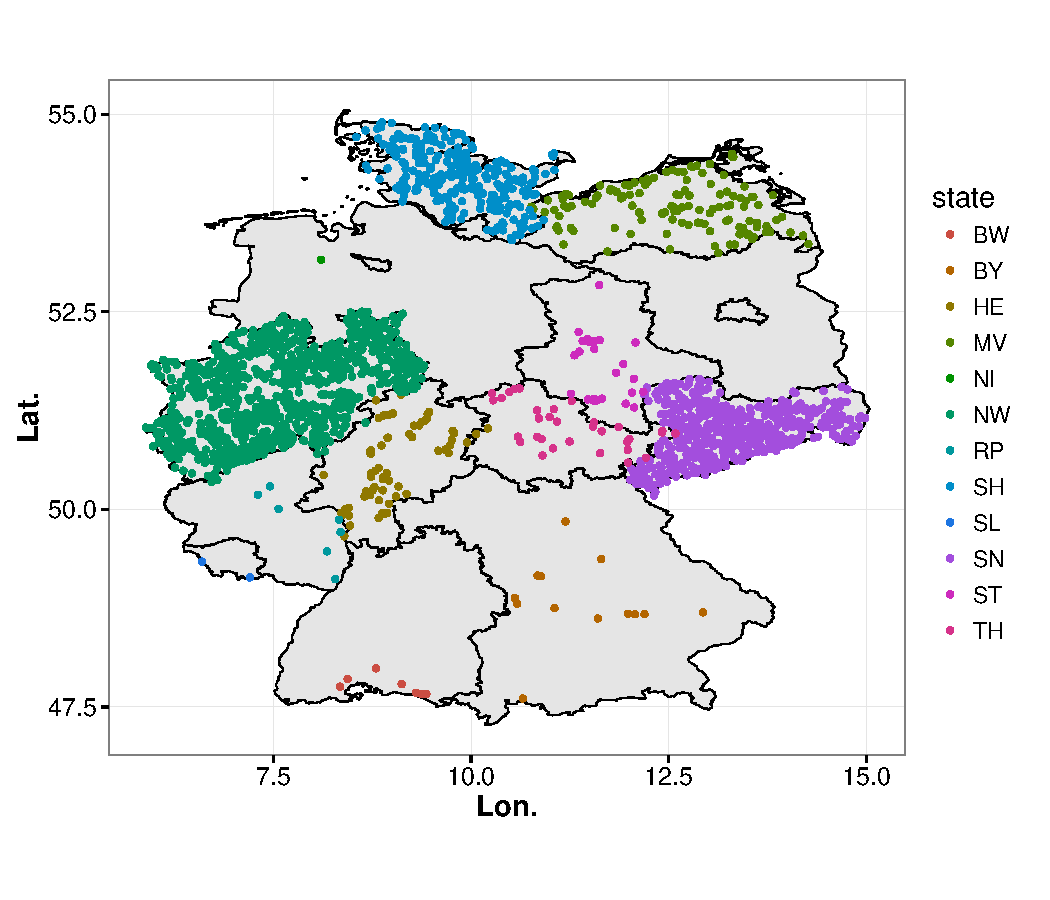
\includegraphics[width=3.33in]{figure1.pdf}
  \caption{Spatial distribution of the 2,301 small stream sampling sites. Colour codes different federal states (see Supplemental Table~S1 for abbreviations).}
  \label{fig:fig1}
\end{figure}

In total 478 different compounds used as pesticides and their metabolites were measured at least once (Supplemental Table~S2). 
Most of the compounds were herbicides (179), followed by insecticides (117) and fungicides (109). % see overview.R
Most samples were taken in the months April till October, while fewer samples were taken during winter (see Supplemental Figure~S2).
We found substantial differences in the spectra of analysed pesticides between federal states (Figure~\ref{fig:fig2}).
The number of analysed pesticides per state ranged from 57 (SL) to 236 (RP) (Supplemental Table~S1). 
4\% (=71,113) of all measurements were concentrations above LOQ.

\begin{figure}[ht]
  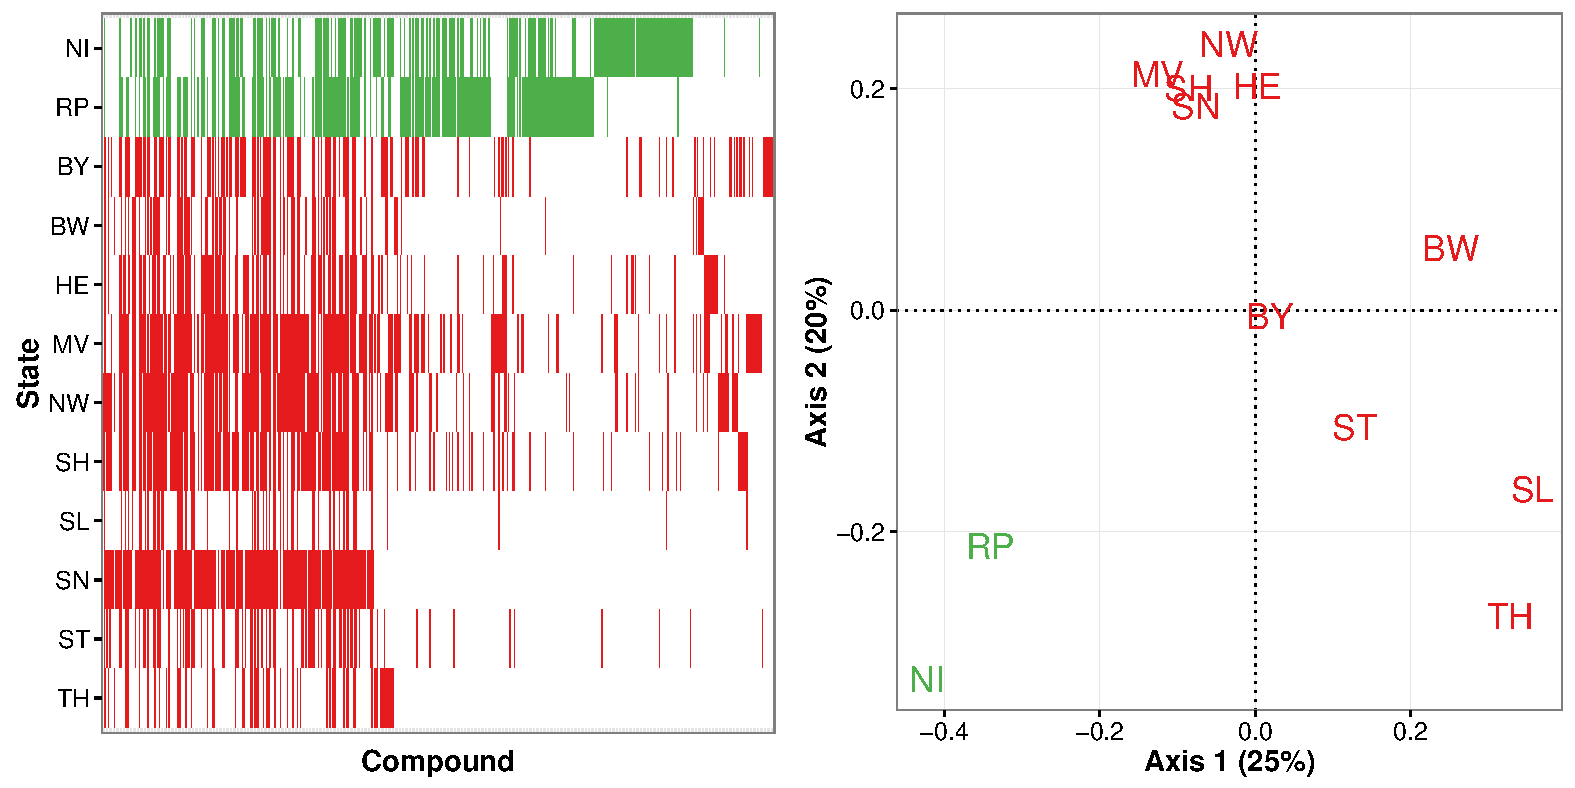
\includegraphics[width=3.33in]{figure2.pdf}
  \caption{Barcode plot of compound spectra of the federal states. Each vertical line is an analysed compound.}
  \label{fig:fig2}
\end{figure}

The distribution of sampling sites across catchment sizes indicated a disproportionally low number of sites with catchments below $10~km^2$, with
most sampling sites having catchment sizes between 10 and 25~$km^2$ (Figure~\ref{fig:fig3}). 


\begin{figure}[ht]
  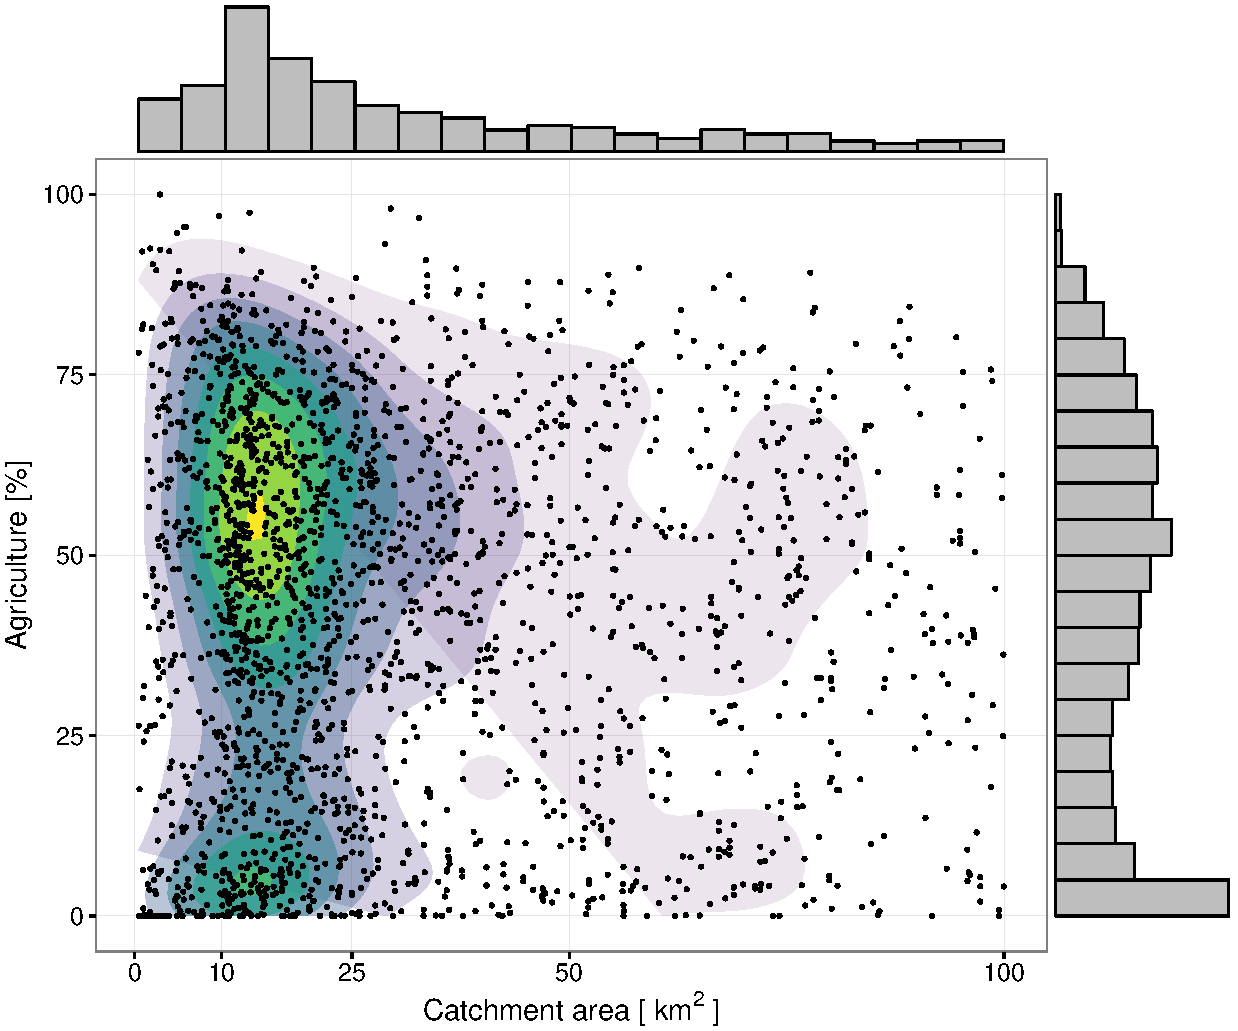
\includegraphics[width=3.33in]{figure3.pdf}
  \caption{Distribution of catchment area across the sampling sites.}
  \label{fig:fig3}
\end{figure}


\subsection{Influence of agricultural land use and catchment size}
We found a positive relationship between agricultural land use and the number of RAC exceedances. 
The non-linear model showed, that below 28\% agriculture the mean number of RAC exceedances dropped statistically significant 3.7-fold from 0.39 (28\% agriculture within the catchment) to 0.10 (no agriculture) (Figure~\ref{fig:fig4}, left).
Catchment size had no statistically significant effect on the number of RAC exceedances (Figure~\ref{fig:fig4}, right).
We also could not detect a statistically significant interaction between catchment size and agriculture. 

\begin{figure}[ht]
  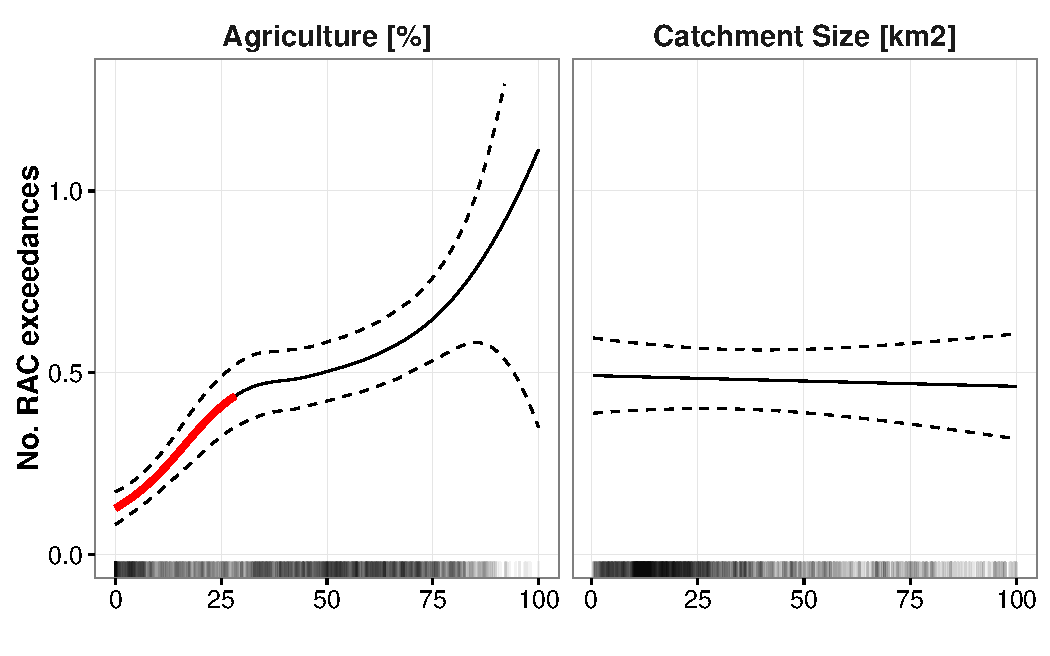
\includegraphics[width=6.5in]{figure4.pdf}
  \caption{Effect of percent agriculture within the catchment (left) and catchment size (right) on the mean number of RAC exceedances per site. Red line marks statistically significant changes. Dashed lines denote 95\% point-wise Confidence Intervals.
  }
  \label{fig:fig4}
\end{figure}


\subsection{Effect of precipitation on pesticide risk}
$prec_{0}$ and $prec_{-1}$ increased the probability of exceeding LOQ and RQ.
In $Q2$ an increase from 0.1~mm to 15~mm of precipitation before sampling ($prec_{-1}$) lead on average to a 43\% higher mean RQ of 0.05 (Supplemental Figure~S7).
The probability to exceed LOQ increases in $Q2$ 1.6-fold from 8.7\% to 13.5\% (Figure~\ref{fig:fig5}). % do_precip.R
Precipitation before sampling ($prec_{-1}$) had a stronger effect than precipitation during sampling ($prec_{0}$) on the probability of exceeding LOQ. 
This difference was less pronounced for the mean value of RQ (Supplemental Figure~S7, top left). 
Moreover, effects differed between individual compounds (see Supplemental Table~S4). 

The first quarter showed the lowest RQ and probability of exceeding LOQ.
Both increased in $Q2$ and decreased towards the end of the year.
There was a 2.5-fold higher probability of exceeding LOQ in $Q2$ (10.6\%) than in $Q1$ (4.6\%) (Figure~\ref{fig:fig5}).
The differences were less pronounced for the mean value of RQ and with less precision  (see Supplemental Figure~S7, left).
Individual compounds showed different temporal patterns (see Supplemental Table~S4). 


\begin{figure}[ht]
  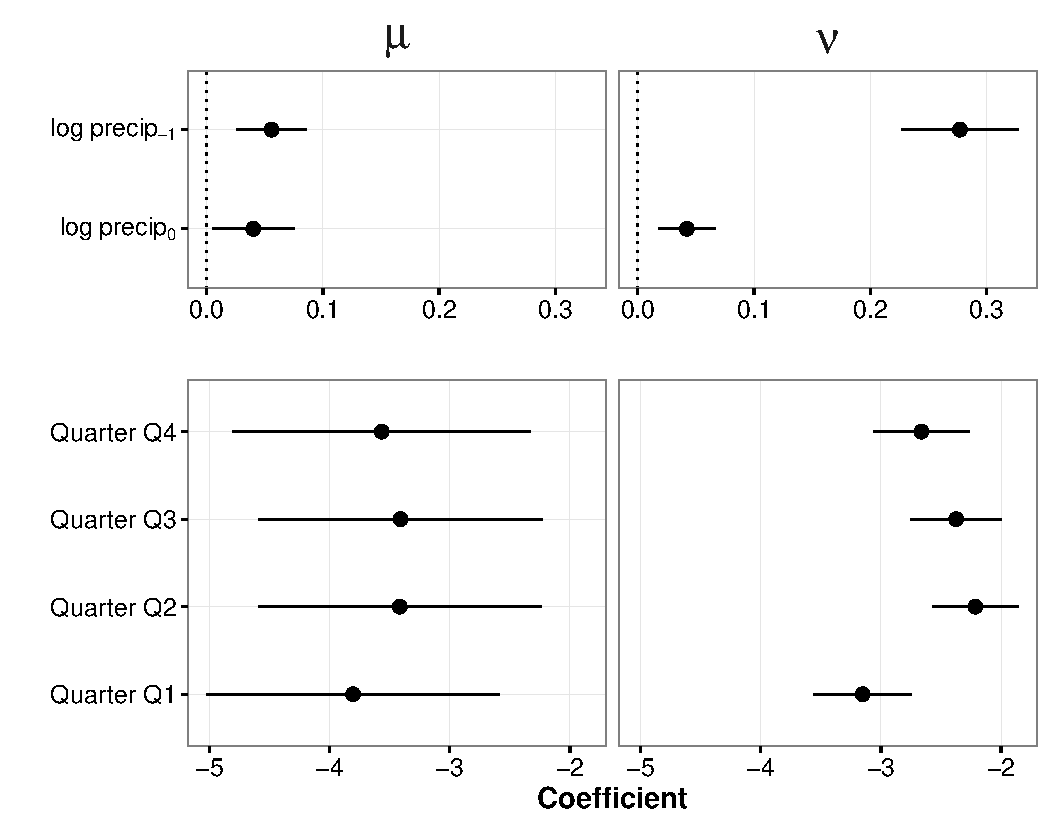
\includegraphics[width=3.33in]{figure5.pdf}
  \caption{Summarised model predictions for the probability to exceed LOQ throughout the year. Black points indicate the probabilities at 0.1 mm precipitation (and their 95\% CI). 
  Orange points indicate the probabilities at 15 mm precipitation.
  Probabilities have been summarised from a meta-analysis of the 22 modelled compounds.
  Single compound coefficients are provided in Supplemental Table~S4 and Figure~S7.
  }
  \label{fig:fig5}
\end{figure}



\subsection{Current pesticide risks in small streams}
We found RAC exceedances in 25.5\% of sampling sites and RQ > 0.1 in 54\% of sites. 
In 23\% of sites none of the chemicals, for which RACs were available, were detected (see also Supplemental Figure~S8).
Neonicotinoid insecticides and Chlorpyrifos showed the highest RQ (Figure~\ref{fig:fig6}). %do_pollution.R
For Thiacloprid and Chlorpyrifos the RAC was equal or less than LOQ, therefore, all detections have a $RQ \ge 1$. 
The herbicides Nicosulfuron and Diflufenican, as well as the fungicide Dimoxystrobin also showed high exceedances of RQ (26.7, 14.1 and 21.1 \% of measurements~\textgreater~LOQ), see also Supplemental Table~S5).
RAC exceedances were found in 14\% of samples with concentrations \textgreater LOQ (and 7.3\% of all samples).

The highest RQs were observed for Chlorpyrifos (max(RQ) = 220), Clothianidin (max(RQ) = 157), Dimoxystrobin(max(RQ) = 117) and Isoproturon (max(RQ) = 80). 
Where analysed, metabolites exhibited the highest detection rates (for example, Metazachlor sulfonic acid was detected in 84\% of all samples where it was analysed (n = 3038, see also Supplemental Figure~S9).
Glyphosate was the compound with the highest detection rates (41\%, n = 3557 samples), followed by Boscalid (23\%, n = 9886) and Isoproturon (22\%, n = 19112). 
However, only the latter showed RAC exceedances (Figure~\ref{fig:fig6}).
In 45.9\% of samples more than one compound was quantified, with a maximum of 54 different compounds in one sample (Supplemental Figure~S10). 

\begin{figure}[ht]
  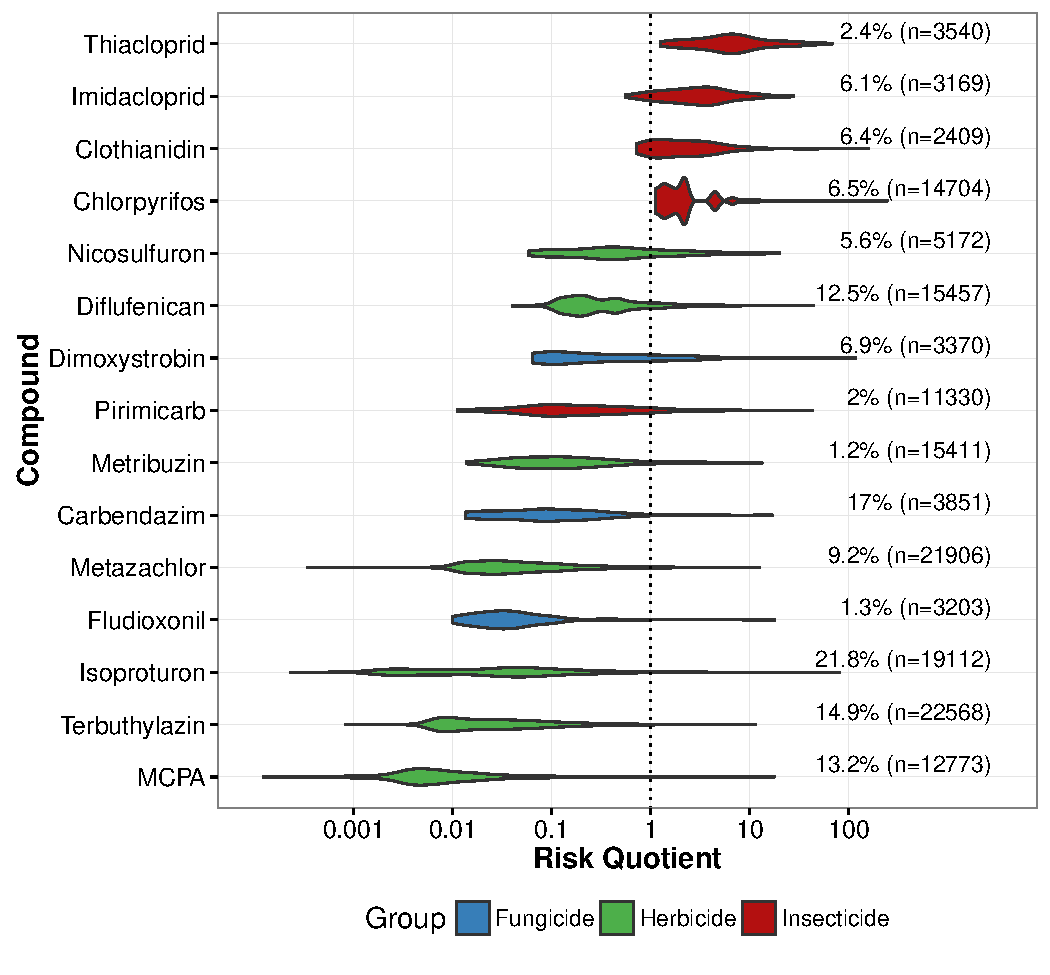
\includegraphics[width=3.33in]{figure6.pdf}
  \caption{15 compounds with the highest observed risk quotients in small streams. Non-detects are not shown due to the logarithmic axis. Numbers on the right give the percentage of values \textgreater LOQ and the total number of samples were the compound was analysed.
  }
  \label{fig:fig6}
\end{figure}




%% -------------------------------------------------------------------------
\section{Discussion}
\subsection{Overview on the compiled dataset}
The compiled dataset of governmental monitoring data, with a particular focus on small streams, represents currently the most comprehensive for Germany.
Similar nationwide datasets have been compiled for the Netherlands \citep{vijver_spatial_2008}, Switzerland \citep{munz_pestizidmessungen_2011} and the United States \citep{stone2014pesticides}.
While the compilations from Europe are of similar quantity and quality to the  data compiled and analysed here, the compilation used in \citet{stone2014pesticides} is much smaller, though these data may be complemented by more data in future analyses. 

% current problems in monitoring and possible solutions
A nationwide assessment of pesticide pollution is hampered by inhomogeneous data across federal states:
Beside large differences in the spatial distribution and quantity of sampling sites (Figure~\ref{fig:fig1}), the spectrum of analysed compounds (Figure~\ref{fig:fig2}) and the quality of chemical analyses differed between states. 
Despite the outlined differences between states, all ecoregions occurring in Germany \citep{illies1978limnofauna,abell2008freshwater} and all major stream types were covered by the data set.
The unequal distribution of sampling sites and the different sampling strategies hamper inference on the total population of small streams in Germany.
We accounted for differences in sampling efforts per site by including the total number of measurement into the statistical models. 
However, we acknowledge that additional differences such as sampling frequency and temporal distribution of the samplings might incur bias between states  \citep{stehle_probabilistic_2013,Xing_Chow_Rees_Meng_Li_Ernst_Benoy_Zha_Hewitt_2013}. 
Consequently, we did not compare the results between states.
Moreover, it is known that differences in analytical quality can influence estimated effects \citep{Martin_Eberle_Nakagaki, Schreiner_Szocs_Bhowmik_Vijver_Schafer_2016}.
However, the used model (Equation~\ref{eqn:eqn3}) explicitly accounted for LOQs and differences therein. 

For Thiacloprid and Chlorpyrifos the LOQs were above the RAC, which means that exceedances are likely underestimated.
For compounds with low RACs a lowering of LOQ through an improvement of chemical analysis is essential for reliable assessment.
Moreover, a nationwide assessment would benefit from a harmonised spectrum of analysed compounds between federal states. 

Given their high abundance in the landscape \citep{nadeau_hydrological_2007} small streams below 10~km\textsuperscript{2} are disproportionally less sampled in current monitoring (Figure~\ref{fig:fig3}), which may be attributed to the missing categorisation in the WFD. 
Clearly, there is currently a lack of knowledge on stressor effects on small streams.
We analysed only data from small streams, however, for lentic small water bodies this lack might be even greater \citep{lorenz_specifics_2016}. 


\subsection{Influence of agricultural land use and catchment size}
% agriculture
As hypothesised, we found a positive relationship between agricultural land use and the number of RAC exceedances.
Especially, we found a statistically significant drop below 28\% of agricultural land use (Figure~\ref{fig:fig4}, left).
This drop indicates that agricultural land use is a major contributor to the observed RAC exceedances.
We note that this drop would have been missed by linear modeling (Supplemental Figure~S5). 
The absence of such a drop would have suggested that other inputs such as from urban gardening are relevant contributors to RAC exceedances.  

% size
We did not find a statistically significant relationship between pesticide pollution and catchment size (Hypothesis 2). 
However, previous studies showed that small streams are more polluted than bigger streams \citep{schulz_field_2004,stehle_pesticide_2015,knauer_pesticides_2016}.
This can be explained by the relatively short gradient of catchment sizes in our dataset, with most of the streams with catchments above $10~km^2$ and below $100~km^2$ (Figure~\ref{fig:fig3}, top).
For example, the gradient of \citet{schulz_field_2004} covered 6 orders of magnitude.


\subsection{Effect of precipitation on pesticide risk}
We found a 36\% higher RQ if samples were taken after rainfall events, which conforms to the hypothesis that run-off is a major input path on the large scale.
However, samples taken on the day of a rainfall event showed less risk than samples taken one day after a rainfall event.
This discrepancy could be explained by a sampling preceding the rainfall event because the temporal resolution of our dataset was 1 day.
Additionally, this might be explained by a delay between the start of a rain event and the peak in discharge or runoff. 

The effects of precipitation were more pronounced for the probability to exceed LOQ, with smaller effect sizes for the absolute value of RQ. 
This may be explained by a higher variability of absolute concentrations.
Overall, our results indicate that current pesticide monitoring relying on grab sampling, largely disconnected from precipitation events, underestimates pesticide risks.
Automatic event-driven samplers \citep{stehle_probabilistic_2013} and passive samplers \citep{fernandez_calibration_2014,moschet_evaluation_2015} may help overcome these shortcomings and provide a better representation of risks.
Our results demonstrate that future monitoring of small water bodies should also capture precipitation events, which is in agreement with other studies \citet{lorenz_specifics_2016}. 

We found the highest the probability of exceeding LOQ from April to June (10\% for Q2) and lowest in the first quarter of the year (4\%, Figure~\ref{fig:fig5}, bottom right).
This annual pattern coincides, as hypothesised, with the main application season for pesticides in Central Europe.
Nevertheless, there are compound-specific differences in the annual pattern, which explains the wide CI for the absolute RQ (Figure~\ref{fig:fig5}, bottom left). 
For example, the herbicide Diflufenican showed the highest RQ and the highest probability of exceeding LOQ during the winter quarters Q1 and Q4 (Supplemental Table~S4), which coincides with the application period it is registered for in Germany \citep{bvl_online_2016}.
Moreover, compound properties, like half-life or water solubility, might influence compound dynamics. 
Our study suggests that pesticide risks display compound specific spatio-temporal dynamics. 
Currently, little is known about these and further research on those might provide useful information for future ecological risk assessment. 
For example, the sensitivity of organisms is often life stage dependent \citep{hutchinson1998analysis} and knowledge on temporal dynamics could inform on concurrent exposure to multiple pesticides, as well as assist to parameterise toxicokinetic and toxicodynamic models \citep{ashauer2016modelling}. 
Moreover, our results show that analysing absolute concentrations and probabilities of LOQ together might deliver valuable insights into risk dynamics.


\subsection{Pesticides in small streams}
Our results suggest that small streams are frequently exposed to ecologically relevant pesticide concentrations.
In one-quarter of small streams RACs were exceeded at least once.
\citet{stehle_pesticide_2015} found the highest percentage of RAC exceedances for organophosphate insecticides. 
By contrast, we found that neonicotinoid insecticides have highest exceedances of RACs, followed by the organophosphate chlorpyrifos. 
This difference can be attributed to the low sample size for neonicotinoid insecticides in their study (n = 33) compared to the dataset presented here (for example 3,540 samples of Thiacloprid, Figure~\ref{fig:fig6}). 
Overall, our results suggest that neonicotinoids may currently pose a high risk to freshwater ecosystems. 
Moreover, our results add further evidence to the growing literature on the risks arising from neonicotinoids for aquatic \citep{morrissey2015neonicotinoid} and terrestrial \citep{pisa2015effects} ecosystems. 

Compared to \citet{stehle_pesticide_2015} we found higher rates of RAC exceedances for insecticides.
They found exceedances in 37.1\% of insecticide measurements \textgreater LOQ (n = 1352, 23 insecticides), whereas, we found exceedances in 67\% of insecticide measurements with RACs \textgreater LOQ (n = 1855, 22 insecticides). 
This could be attributed to different insecticides considered and different underlying RACs.
Our study has only 7 insecticides with RACs in common with the insecticides investigated by \citet{stehle_pesticide_2015}.
Moreover, all RACs were lower in our study (average difference = -0.71 $\mu g/L$, range = [-2.757; -0.005]). 
Nevertheless, it must be noted that the dataset compiled here comprised only samples from grab sampling, which may considerably underestimate pesticide exposure \citep{stehle_probabilistic_2013, Xing_Chow_Rees_Meng_Li_Ernst_Benoy_Zha_Hewitt_2013}. 

By contrast, \citet{knauer_pesticides_2016} found exceedances from monitoring data mainly for herbicides and fungicides and only one insecticide Chlorpyrifos-methyl.
Moreover, RAC exceedances in Switzerland were generally lower and less abundant (for example 6 exceedances (=0.2\%) for Isoproturon with a maximum RQ of 2) compared to our results for Germany. 
This might reflect differences in pesticide use between countries, ecoregions and RACs used. 
From the definition of RAC it follows that if the concentration of a compound exceeds its RAC ecological effects are expected.
Indeed, \citet{stehle_agricultural_2015} found that the biological diversity of stream invertebrates was significantly reduced by 30\% at RQ = 1.12 and by 10\% at 1/10 of RAC.
We found RQ values greater than 1.12 in 25\% of small streams and RQ at 1/10 of RAC in 54\% of small streams. 
Consequently, we conclude that agricultural pesticides are on a large scale a major threat to small streams, the biodiversity they host and the services they provide. 
This threat may exacerbate because pesticides often occur in mixtures \cite{schreiner_pesticide_2016} and may co-occur with other stressors \citep{schafer_contribution_2016}. 

% Approval / Risk Assessment
Monitoring data, despite the outlined limitations, provides an opportunity to study large-scale environmental occurrence patterns of pesticides.
Furthermore, such nationwide compilations, may not only be used for governmental surveillance, but also to answer other questions, like validation of exposure modelling \cite{knabel_fungicide_2014}, retrospective evaluation of regulatory risk assessment \citep{knauer_pesticides_2016,stehle_pesticide_2015}or occurrences of pesticide mixtures \cite{schreiner_pesticide_2016}.
However, the sampling design needs to account for precipitation events to provide robust data. 
Our results suggest that exceedances of RACs are landscape dependent % = Zusammenhang RAC<->Agriculture
and therefore, pesticide regulation should account for landscape features. 
Moreover, the high exceedances of RACs indicate that greater efforts are needed to describe causal links, which may lead to further developments of the current authorisation procedure.



%%%%%%%%%%%%%%%%%%%%%%%%%%%%%%%%%%%%%%%%%%%%%%%%%%%%%%%%%%%%%%%%%%%%%
\begin{acknowledgement}
The authors thank the federal state authorities and the German Working Group on water issues of the Federal States (LAWA) for providing chemical monitoring data and the German Environment Agency (UBA) for funding a related project (FKZ 3714 67 4040 / 1). 
We thank Alexandra Müller, Wolfram König and Volker Mohaupt (German Environment Agency (UBA)), Martin Keller and Beate Bänsch-Baltruschat (German Federal Institute of Hydrology (BfG)), Matthias Liess and Kaarina Foit (Center for Environmental Research (UFZ)) for their contributions to this project. 
\end{acknowledgement}


%%% Word count
% abstract    :  200
% 1 big(600)  :  600
% 5 small(300): 1500
% acknowledg  :   80
%              =====
% subtotal      2380
% text body   : 3962
% ======================================
% subtotal    : 6342
% - captions  :  200
% =========================================
% total       : 6142

%%%%%%%%%%%%%%%%%%%%%%%%%%%%%%%%%%%%%%%%%%%%%%%%%%%%%%%%%%%%%%%%%%%%%
\begin{suppinfo}
The following files are available free of charge.
\begin{itemize}
  \item Supplemental\_Materials.pdf : Supplemental Materials (Figures, Tables, Models).
\end{itemize}
\end{suppinfo}


%%%%%%%%%%%%%%%%%%%%%%%%%%%%%%%%%%%%%%%%%%%%%%%%%%%%%%%%%%%%%%%%%%%%%
\bibliography{references}

\end{document}
